\documentclass[11pt,a4paper]{article}

% ── Rubric-fixed layout (INVIOLABLE) ───────────────────────────────
% Margins 2.5cm, 11pt, line spacing 1.15, max 10 pages of body.
\usepackage[a4paper,margin=2.5cm]{geometry}
\usepackage{setspace}
\setstretch{1.15}

% ── Encoding & language ───────────────────────────────────────────
\usepackage[utf8]{inputenc}
\usepackage[T1]{fontenc}
\usepackage[english]{babel}
\usepackage{microtype}

% ── Font: Helvetica (sans-serif) ──────────────────────────────────
\usepackage[scaled=0.95]{helvet}
\renewcommand{\familydefault}{\sfdefault}

% ── Colour palette ────────────────────────────────────────────────
\usepackage[table,xcdraw]{xcolor}
\definecolor{novagreen}{RGB}{100,155,0}
\definecolor{darkgray}{RGB}{60,60,60}
\definecolor{lightgray}{RGB}{245,245,245}

% ── Headers / footers ─────────────────────────────────────────────
\usepackage{fancyhdr}
\pagestyle{fancy}
\fancyhf{}
\fancyhead[L]{\footnotesize\textcolor{darkgray}{Genetic Algorithm --- Group 36 Divergence}}
\fancyhead[R]{\footnotesize\textcolor{darkgray}{NOVA IMS $\cdot$ CIfO 2025/2026}}
\fancyfoot[C]{\footnotesize\thepage}
\renewcommand{\headrulewidth}{0.4pt}
\renewcommand{\footrulewidth}{0pt}

% ── Section styling (novagreen) ───────────────────────────────────
\usepackage{titlesec}
\titleformat{\section}
  {\bfseries\color{novagreen}}{\thesection}{0.8em}{}
\titleformat{\subsection}
  {\color{novagreen}}{\thesubsection}{0.8em}{}
\titleformat{\subsubsection}
  {\bfseries\color{darkgray}}{\thesubsubsection}{0.8em}{}
\titlespacing*{\section}{0pt}{8pt}{4pt}
\titlespacing*{\subsection}{0pt}{6pt}{3pt}
\titlespacing*{\subsubsection}{0pt}{4pt}{2pt}

% ── Math ──────────────────────────────────────────────────────────
\usepackage{amsmath, amssymb}

% ── Graphics / floats ─────────────────────────────────────────────
\usepackage{graphicx}
\usepackage{float}
\usepackage{placeins}

% ── Tables (booktabs + green header macros) ───────────────────────
\usepackage{booktabs}
\usepackage{multirow}
\usepackage{array}
\usepackage{tabularx}
\usepackage{colortbl}
\newcommand{\tH}[1]{\textcolor{novagreen}{\textbf{#1}}}
\newcommand{\gmid}{\arrayrulecolor{novagreen}\midrule\arrayrulecolor{black}}

% ── Captions ──────────────────────────────────────────────────────
\usepackage{caption}
\captionsetup{font=small, labelfont={bf,color=novagreen}, skip=4pt}

% ── Lists (novagreen bullets) ─────────────────────────────────────
\usepackage{enumitem}
\setlist[itemize]{noitemsep, topsep=2pt, parsep=0pt, partopsep=0pt,
                  leftmargin=1.4em, label=\textcolor{novagreen}{\textbullet}}

% ── Paragraph spacing ─────────────────────────────────────────────
\setlength{\parindent}{0pt}
\setlength{\parskip}{3pt}

% ── Hyperlinks ────────────────────────────────────────────────────
\usepackage[colorlinks=true, linkcolor=novagreen, citecolor=darkgray,
            urlcolor=novagreen, pdfborder={0 0 0}]{hyperref}

% ── Convenience ───────────────────────────────────────────────────
\newcommand{\ttt}[1]{\texttt{\hyphenchar\font=`\-\relax #1}}

\begin{document}

% ============================================================
% Cover page
% ============================================================

\begin{titlepage}
\thispagestyle{empty}
\centering
\vspace*{1.5cm}

{\small\color{darkgray} Master's in Data Science \& Advanced Analytics}\\[2pt]
{\small\color{darkgray} Computational Intelligence for Optimization $\cdot$ 2025/2026}
\vspace{1.5cm}

{\color{novagreen}\rule{\linewidth}{2pt}}\\[10pt]
{\LARGE\bfseries\color{darkgray} A Genetic Algorithm Approach\\[6pt]
to Image Reconstruction}\\[10pt]
{\large\color{darkgray} Reconstructing Vermeer's \textit{Girl with a Pearl Earring}}\\[10pt]
{\color{novagreen}\rule{\linewidth}{2pt}}
\vspace{2cm}

{\small\bfseries\color{darkgray} GROUP 36 --- DIVERGENCE}\\[0.8em]
{\small\color{darkgray}
  \begin{tabular}{ll}
    Bárbara Franco           & 20250388 \\[4pt]
    Catarina Mendinhas       & 20250422 \\[4pt]
    Maria Miguel Fonseca     & 20250380 \\[4pt]
    Tiago Antunes            & 20250357 \\[4pt]
  \end{tabular}
}
\vfill

{\small\color{darkgray} Source code:
\href{https://github.com/barbara-sousa-franco/cifo_project}{github.com/barbara-sousa-franco/cifo\_project}}\\[8pt]
{\small\color{darkgray} NOVA Information Management School (NOVA IMS)}\\[4pt]
{\small\color{darkgray} May 2026}
\vspace{0.4cm}\\
{\color{novagreen}\rule{\linewidth}{1pt}}

\end{titlepage}



% ============================================================
% TABLE OF CONTENTS
% ============================================================
\tableofcontents
\thispagestyle{empty}
\newpage

% ============================================================
% Report starts here
% ============================================================
\setcounter{page}{1}


\section{Executive Summary}

We reconstruct Vermeer's \textit{Girl with a Pearl Earring}
using a genetic algorithm operating on a fixed budget of 100 semi-transparent
triangles. A One-Factor-At-A-Time (OFAT) protocol, followed by a random
search over the surviving hyperparameters, identified the following
winning configuration: Adaptive Mutation Schedule, Uniform Crossover,
mutation probability $p_m \approx 0.012$, crossover probability
$p_c \approx 0.99$, triangle-size cap $\approx 0.57$, alpha window
$[0.18, 0.52]$, tournament size $k = 5$, and Restricted Mating with
distance window $[0.010, 0.348]$. On the calibration budget
(population $100$, $500$ generations, $15$ runs) the mean final RMSE
dropped from $30.18$ (best fully-configured GA without diversity mechanisms)
to $26.56$ after all enhancements were combined -- a $12\%$ improvement
over that baseline, or a $36\%$ improvement relative to the strongest
mutation-only configuration ($41.75$). The final long-budget run
(population $500$, $15{,}000$ generations) reached \textbf{(PENDING:
final\_run RMSE)} and is reported in \S6.
As a Challenge extension, the perceptual CIEDE2000 metric reached
$\Delta E_{00} = 6.20$ on a shorter budget (POP $= 200$, GENS $= 5{,}000$).


\section{Introduction \& Problem Formalization}

\begin{figure}[H]
\centering
\begin{minipage}{0.30\linewidth}
  \centering
  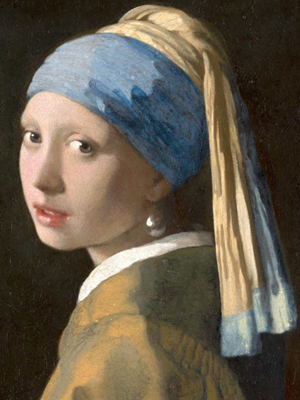
\includegraphics[width=\linewidth]{girl_pearl_earing.png}\\[2pt]
  {\footnotesize\textit{Target}}
\end{minipage}\hspace{0.04\linewidth}%
\begin{minipage}{0.30\linewidth}
  \centering
  
\includegraphics[width=\linewidth]{ciede2000_short_best_challenge_short.png}\\[2pt]
  {\footnotesize\textit{Best CIEDE2000 (\S7)}}
\end{minipage}
\caption{Vermeer's \textit{Girl with a Pearl Earring} ($300\times 400$
target) and the best reconstruction obtained by our GA under the
CIEDE2000 perceptual metric ($\Delta E_{00} = 6.20$). Both are
composed of exactly 100 semi-transparent triangles.}
\label{fig:teaser}
\end{figure}

In this work, we address the problem of reconstructing the painting \textit{Girl with a Pearl Earring} by Johannes Vermeer using genetic algorithms. The search space is highly dimensional, and solution quality can be directly assessed through visual inspection.

Each candidate solution, or \textit{Individual}, consists of an ordered list of 100 triangles. Each triangle is encoded by 10 normalized real-valued genes:

\vspace{-0.6em}
\[
t = (x_{1}, y_{1}, x_{2}, y_{2}, x_{3}, y_{3}, r, g, b, a)
\]
\vspace{-0.8cm}

The vertex coordinates are mapped to image space using the target image dimensions (300 × 400), while color and opacity values are scaled to the range [0,255]. Keeping all genes normalized to [0,1] allows mutation and crossover operators to act uniformly across all parameters.

The phenotype is generated by sequentially rendering the triangles onto a black RGBA canvas using Porter–Duff alpha compositing. As a result, later triangles visually overlap earlier ones, implicitly defining a painting order.

Fitness is evaluated through the pixel-wise \textbf{Root Mean Squared Error} (RMSE) between the rendered image and the target painting. As an extension, we also evaluate \textbf{CIEDE2000}, a perceptually uniform color-distance metric computed in CIE Lab space, which better reflects human perception of color differences.

To avoid invalid or visually meaningless primitives, triangles are constrained by maximum size, opacity bounds, and positive area requirements. Degenerate triangles are corrected through small vertex perturbations, while oversized triangles are contracted toward their centroid.



\section{Methodology}

\subsection{Genetic Algorithm}

A standard generational Genetic Algorithm
\cite{eibensmith2015} was implemented. The algorithm starts with an initial
population and, over a predefined maximum number of generations, iteratively
creates new populations by selecting parents using the chosen selection
method and applying crossover and mutation according to the specified
probabilities. When elitism is enabled, the best individual from the current
generation is copied unchanged into the next generation, ensuring that the
highest-quality solution found so far is preserved. Additionally, the best
individual and its corresponding fitness value from each generation are
stored to allow analysis of the algorithm's evolutionary progress over time.


\subsection{Mutation Operators}

Four mutation operators were implemented and compared:

\vspace{0.2cm}

\textbf{VCF Mutation (Vertex, Color, Full, Order)}: Each of the 100 triangles mutates with probability $p_m$. If selected, the triangle randomly draws a subset of one to four mutation types to apply simultaneously. A \textit{vertex mutation} perturbs one randomly chosen vertex by Gaussian noise ($\sigma=0.05$). A \textit{color mutation} perturbs all RGBA channels by Gaussian noise ($\sigma=0.05$), with alpha re-clipped to $[\alpha_{\min}, \alpha_{\max}]$. A \textit{full mutation} replaces the triangle entirely with a new random one and skips any other type. An \textit{order mutation} swaps the triangle with an overlapping neighbour, altering the compositing stack without modifying any gene values, because rendering order determines which triangles occlude others.
\vspace{0.2cm}


\textbf{Full Replacement Mutation} : Each triangle is replaced with a new random triangle with a probability of $p_{m}$. It is the most destructive one.

\vspace{0.2cm}

\textbf{Gaussian Gene Mutation}: Each of the 10 genes of each triangle is independently perturbed by $\mathcal{N}(0, \sigma)$ with $\sigma=0.05$. Domain constraints are re-applied after perturbation. This mutation explores the genome uniformly.

\textbf{Color Creep Mutation}: Only the four RGBA channels (genes 6--9) are perturbed, leaving vertex geometry unchanged. Designed for late-stage refinement when triangle placement is approximately correct but colors require fine-tuning. In this case, $p_{m}$ is the probability of changing each RGBA channel, not the probability of mutating the triangle.

\vspace{0.2cm}

Additionally, an \textbf{Adaptive Mutation Schedule} was also implemented, switching operators by generation phase: Full Replacement for the first $40\%$ generations, Gaussian for generations $40-85\%$, and Color Creep for the final $15\%$.



\subsection{Crossover Operators}

Four crossover operators were implemented and compared, all of them perform crossover with probability $p_{c}$:

\vspace{0.2cm}

\textbf{Uniform crossover}: Each gene is inherited independently from parent 1 (probability $p$) or parent 2 (probability $1-p$), with the default value for $p$ being $0.5$. The two
offspring are complementary: wherever child~1 inherits from parent~1, child~2
inherits from parent~2. This maximises mixing but may disrupt contiguous
blocks of well-placed triangles.

\vspace{0.2cm}

\textbf{K-Point Crossover}: $K$ cut points are chosen uniformly at random
from $\{1,\ldots,N-1\}$, where $K\sim\mathrm{Uniform}(k_{\min},k_{\max})$
with $k_{\min}=3$, $k_{\max}=7$. Segments between consecutive cut points are
alternately assigned from each parent, preserving contiguous triangle blocks
while allowing more recombination than single-point.
\vspace{0.2cm}

\textbf{Reduced Surrogate Crossover}: The cut point is restricted to
positions where the two parents differ, ensuring that every crossover event
produces offspring that are genuinely distinct from both parents. If fewer
than two differing positions exist, the parents are returned unchanged.

\vspace{0.2cm}

\textbf{Shuffle Crossover}: Both parents are permuted by the same random
shuffle before single-point crossover; the inverse permutation is then applied
to the offspring. This eliminates positional bias, the tendency for
early-genome triangles to always co-inherit, without the disruptive character
of uniform crossover.

\vspace{0.2cm}
Additionally, an \textbf{Adaptive Crossover Schedule} was implemented,
switching operator based on evolutionary stage: Uniform for the first $50\%$
of generations, when little useful structure has yet emerged and broad
exploration is beneficial; K-Point for generations $50$--$85\%$, providing
structured mixing as good triangle blocks consolidate; and Reduced Surrogate
for the final $15\%$, restricting recombination to positions where the parents
genuinely differ and thereby preserving near-converged solutions.


\subsection{Diversity Preservation Mechanisms}
Four mechanisms for maintaining population diversity were
implemented and evaluated:
\vspace{0.2cm}

\textbf{Adaptive Mutation Rate} (Rechenberg's 1/5 Rule
\cite{rechenberg1973}): A sliding window
of $w=10$ generations tracks the fraction of offspring that improve on their
parents. If this success rate exceeds $0.2$, $p_m$ is scaled up by $10\%$;
if below $0.2$, it is scaled down by $10\%$, clipped to
$[p_{\min}, p_{\max}]=[0.001, 0.5]$.
\vspace{0.2cm}

\textbf{Diversity Injection}: The fitness standard deviation across the
population is monitored as a phenotypic diversity proxy. When it drops below
a threshold fraction of the initial standard deviation, the worst
$d_{\text{frac}}$ of individuals are replaced with new random ones, injecting
fresh genetic material without discarding the elite.
\vspace{0.2cm}

\textbf{Fitness Sharing}: Each individual's fitness is adjusted by a crowding
factor computed from pairwise genotypic distances (Euclidean over the
flattened 1\,000-gene vector, normalised by $\sqrt{1000}$). For minimisation,
the adjusted fitness is $\tilde{f}(i) = f(i)\cdot(1 + \lambda \cdot
c(i))$, where $c(i)$ is the mean sharing coefficient within niche radius
$\sigma_{\text{share}}$ and $\lambda$ controls the penalisation strength.
Tournament selection then operates on $\tilde{f}$, making individuals in
densely populated genotype regions appear less attractive.
\vspace{0.2cm}

\textbf{Restricted Mating} \cite{goldberg1989, eshelman1991}: Parent~2 is
constrained to candidates whose genotypic distance to parent~1 falls within
$[d_{\min}, d_{\max}]$, preventing both inbreeding (near-identical parents
produce no new material) and incompatible crossings (very distant parents
destroy useful structure). A pool of candidates is sampled first; if none
satisfies the distance window, the candidate closest to the midpoint
$\tfrac{d_{\min}+d_{\max}}{2}$ is selected as a fallback.


\section{Experimental Setup}

In this project, a series of experiments was conducted, with their configurations summarized in the table below.

\begin{table}[h]
\centering
\begin{tabular}{lccc}
\toprule
\tH{Experiment} & \tH{Pop Size} & \tH{Max Gens} & \tH{N Runs} \\
\gmid
Mutation Comparison & 100 & 500 & 15 \\
Crossover Comparison & 100 & 500 & 15 \\
Probability sweep & 100 & 500 & 15 \\
Triangle Size limits & 100 & 500 & 15 \\
Alpha windows & 100 & 500 & 15  \\
Diversity mechanisms & 100 & 500 & 15  \\
Final run & 500 & 15000 & 01  \\
\bottomrule
\end{tabular}
\caption{Experimental configuration summary}
\end{table}

During the experimental phase, reduced population sizes and generation limits were adopted to decrease computational cost and enable efficient parameter evaluation. For the final execution, both parameters were increased to provide the genetic algorithm with a larger search budget, allowing improved convergence and finer solution optimization. In this stage, only a single run was conducted, since the purpose was not comparative evaluation but rather the generation of the best achievable solution.

The first and second experimental phases are independent, given that the first was executed with $p_c = 0$ and the second with $p_m = 0$. The subsequent experimental stages are inherently dependent on the outcomes of the previous ones, as they incorporate the best-performing operators and parameter settings obtained in earlier experiments.

\section{Results}

\subsection{Mutation Comparison}

With crossover disabled, a Kruskal-Wallis test confirmed
statistically significant differences among operators ($H = 61.21$, $p < 0.0001$).

\begin{table}[h]
\centering
\begin{tabular}{lcccc}
\toprule
\tH{Operator} & \tH{Mean} & \tH{Std} & \tH{Best} & \tH{Worst} \\
\gmid
AdaptiveMut & 41.75 & 1.17 & 39.58 & 43.98 \\
Gaussian    & 43.16 & 1.09 & 40.89 & 45.23 \\
ColorCreep  & 49.48 & 1.97 & 45.57 & 53.62 \\
VCF         & 49.75 & 1.40 & 47.88 & 53.08 \\
Full        & 52.13 & 1.26 & 50.40 & 54.60 \\
\bottomrule
\end{tabular}
\caption{Mutation operator comparison - mean final RMSE over 15 runs}
\end{table}

The Adaptive Mutation Schedule achieved the lowest mean RMSE, significantly
outperforming all standalone operators ($p \leq 0.0037$). Gaussian was the
best standalone operator, while ColorCreep and VCF showed no statistically
significant difference between them ($p = 0.8035$). Full Replacement performed
worst, as its high destructiveness prevents the accumulation of improvements
across generations. ColorCreep's underperformance as a standalone operator is expected since
it only perturbs colour channels and triangle geometry remains frozen at
random initialisation for all 500 generations. In the Adaptive Schedule,
this limitation is avoided because Gaussian mutation has already shaped
the geometry before ColorCreep takes over for final colour refinement
(see Figure~\ref{fig:mutation_comparison} in the appendix).
Based on these results, the Adaptive Mutation Schedule was selected as the
fixed mutation operator for all subsequent experiments.

\subsection{Crossover Comparison}
With mutation disabled, a Kruskal-Wallis test confirmed
statistically significant differences among operators ($H = 46.24$, $p < 0.0001$).

\begin{table}[h]
\centering
\begin{tabular}{lcccc}
\toprule
\tH{Operator} & \tH{Mean} & \tH{Std} & \tH{Best} & \tH{Worst} \\
\gmid
Uniform          & 51.06 & 1.32  & 49.41 & 53.86 \\
AdaptiveXO       & 51.07 & 1.34  & 49.41 & 53.89 \\
Shuffle          & 52.36 & 1.71  & 50.01 & 55.19 \\
KPoint           & 53.41 & 1.69  & 50.79 & 57.31 \\
ReducedSurrogate & 58.68 & 1.19  & 56.97 & 61.32 \\
\bottomrule
\end{tabular}
\caption{Crossover operator comparison - mean final RMSE over 15 runs}
\end{table}

Uniform crossover achieved the lowest mean RMSE, statistically tied with
Adaptive XO ($p = 0.836$). Both significantly outperformed K-Point, Shuffle
and Reduced Surrogate ($p \leq 0.038$). Reduced Surrogate was the weakest:
restricting cuts to differing positions becomes counter-productive when
parents are still highly heterogeneous, which is most of the time on a
continuous representation. Adaptive XO matched Uniform without improving on
it, suggesting that the late-stage Reduced Surrogate stage is neutral once
Uniform has already explored the genome. We selected Uniform as the fixed
crossover operator for subsequent phases (see Figure~\ref{fig:crossover_comparison} in the appendix).

\subsection{Mutation and Crossover Probability Search}

With the operators fixed, we ran a $3 \times 3$ grid over
$p_m \in \{0.01, 0.05, 0.15\}$ and $p_c \in \{0.85, 0.90, 0.95\}$, 15 runs
each. The Kruskal-Wallis test confirmed strongly significant differences
across the nine cells ($H = 107.78$, $p < 0.0001$).

\begin{table}[h]
\centering
\begin{tabular}{lcccc}
\toprule
\tH{Configuration} & \tH{Mean} & \tH{Std} & \tH{Best} & \tH{Worst} \\
\gmid
$p_m=0.01,\ p_c=0.95$ & 31.48 & 0.75 & 30.10 & 33.30 \\
$p_m=0.01,\ p_c=0.90$ & 31.72 & 0.62 & 30.97 & 33.03 \\
$p_m=0.01,\ p_c=0.85$ & 31.94 & 0.77 & 30.30 & 33.29 \\
$p_m=0.05,\ p_c=0.95$ & 32.90 & 0.79 & 31.53 & 34.63 \\
$p_m=0.05,\ p_c=0.90$ & 32.94 & 0.75 & 32.05 & 34.33 \\
$p_m=0.05,\ p_c=0.85$ & 33.16 & 0.82 & 31.61 & 34.87 \\
$p_m=0.15,\ p_c=0.90$ & 35.84 & 0.68 & 34.19 & 36.84 \\
$p_m=0.15,\ p_c=0.95$ & 36.37 & 0.91 & 34.94 & 38.01 \\
$p_m=0.15,\ p_c=0.85$ & 36.76 & 1.19 & 35.42 & 39.74 \\
\bottomrule
\end{tabular}
\caption{Mutation/crossover probability sweep - mean final RMSE over 15 runs}
\end{table}

The mutation rate is the dominant factor: $p_m=0.01$ clearly beats $p_m=0.05$
($p \leq 0.0008$), which in turn beats $p_m=0.15$ ($p \leq 5 \times 10^{-6}$).
Within each $p_m$ band the three $p_c$ values are statistically
indistinguishable ($p \geq 0.115$), so the choice of $p_c=0.95$ is within
noise; we kept it for consistency with the lowest-mean cell. The clean
clustering of the nine cells into three $p_m$ bands is visually evident
in Figure~\ref{fig:probabilities_comparison} (appendix).

\subsection{Maximum Triangle Size}

We constrained the bounding-box span of each triangle to a
cap $s_{\max}$ applied independently on each axis of the normalised genome
space (so $s_{\max}=0.4$ means the triangle can span at most $40\%$ of the
canvas in either $x$ or $y$). Triangles whose proposed span exceeds the cap
are contracted toward their centroid, preserving shape. We tested
$s_{\max} \in \{1.0, 0.4, 0.25, 0.15\}$. Kruskal-Wallis: $H = 51.14$,
$p < 0.0001$.

\begin{table}[h]
\centering
\begin{tabular}{lcccc}
\toprule
\tH{$s_{\max}$} & \tH{Mean} & \tH{Std} & \tH{Best} & \tH{Worst} \\
\gmid
1.00 & 31.48 & 0.75 & 30.10 & 33.30 \\
0.40 & 32.01 & 0.43 & 31.37 & 32.64 \\
0.25 & 36.96 & 0.65 & 35.83 & 38.51 \\
0.15 & 53.84 & 1.26 & 51.79 & 55.90 \\
\bottomrule
\end{tabular}
\caption{Maximum triangle size - mean final RMSE over 15 runs}
\end{table}

Removing the size cap ($s_{\max}=1.0$) wins by a small but significant margin
over $0.40$ ($p = 0.023$), and very large margins below that. With only 100
primitives, the GA needs to be able to paint large regions (the background,
the head outline) in a single triangle; aggressive caps force the population
to waste capacity tiling these regions. The drop from $0.25$ to $0.15$ is
dramatic (+17 RMSE), confirming this argument. We adopted $s_{\max}=1.0$;
convergence curves and best-individual renderings per cap are reported in
Figures~\ref{fig:triangle_graphs} and~\ref{fig:triangle_images} (appendix).

\subsection{Alpha Windows}

Triangles' alpha channel was constrained to a window
$[\alpha_{\min}, \alpha_{\max}]$, tested for five windows. Kruskal-Wallis:
$H = 48.62$, $p < 0.0001$.

\begin{table}[h]
\centering
\begin{tabular}{lcccc}
\toprule
\tH{Window} & \tH{Mean} & \tH{Std} & \tH{Best} & \tH{Worst} \\
\gmid
$[0.10, 0.40]$ & 30.18 & 0.54 & 29.36 & 31.19 \\
$[0.00, 1.00]$ & 31.48 & 0.75 & 30.10 & 33.30 \\
$[0.30, 0.80]$ & 31.94 & 0.75 & 30.96 & 33.24 \\
$[0.20, 0.90]$ & 31.95 & 0.59 & 30.66 & 33.22 \\
$[0.50, 0.70]$ & 33.15 & 0.79 & 31.90 & 35.26 \\
\bottomrule
\end{tabular}
\caption{Alpha window comparison - mean final RMSE over 15 runs}
\end{table}

A narrow, low-alpha window $[0.10, 0.40]$ dominates the unconstrained baseline
by $1.3$ RMSE ($p < 0.0001$). Translucent triangles favour additive layering:
a region's colour emerges from several overlapping primitives rather than a
single opaque one, which raises the effective resolution of the palette
without increasing the chromosome size. Pushing alpha higher
($[0.20, 0.90]$, $[0.30, 0.80]$) eliminates this advantage, and the very
narrow high-alpha window $[0.50, 0.70]$ is the worst configuration. We fixed
the window at $[0.10, 0.40]$ (see Figure~\ref{fig:alpha_comparison} in
the appendix for convergence curves and final-fitness distributions).

\subsection{Diversity Preservation Mechanisms}

The four mechanisms described in \S3.4 were evaluated against
the baseline (winners so far + plain tournament selection), individually and
in two combinations. Kruskal-Wallis: $H = 76.78$, $p < 0.0001$.

\begin{table}[h]
\centering
\begin{tabular}{lcccc}
\toprule
\tH{Mechanism} & \tH{Mean} & \tH{Std} & \tH{Best} & \tH{Worst} \\
\gmid
Restricted Mating          & 27.59 & 0.56 & 26.64 & 28.71 \\
Sharing + Restricted Mating & 27.63 & 0.62 & 26.23 & 28.78 \\
Baseline (no mechanism)    & 30.18 & 0.54 & 29.36 & 31.19 \\
Diversity Injection        & 30.25 & 0.40 & 29.62 & 31.07 \\
Fitness Sharing            & 30.32 & 0.50 & 29.32 & 31.12 \\
Adaptive Mutation Rule     & 30.75 & 0.63 & 29.56 & 31.59 \\
Adaptive + Injection       & 31.28 & 0.63 & 29.86 & 32.29 \\
\bottomrule
\end{tabular}
\caption{Diversity mechanisms - mean final RMSE over 15 runs}
\end{table}

Restricted mating was the only mechanism that produced a substantial
improvement, cutting $2.59$ RMSE points relative to the baseline
($p < 0.0001$). Adding fitness sharing on top did not help ($p = 0.74$,
statistically tied with Restricted Mating alone), so we kept just
Restricted Mating for parsimony. The other mechanisms either matched
the baseline (Fitness Sharing, Diversity Injection) or slightly hurt
(Adaptive Mutation Rule, Adaptive + Injection). A sanity-check run
combining all four mechanisms (\textit{all\_combined}: avg $32.45$, std
$0.60$) confirmed that aggregating them is strictly worse than using
only the one that works. The dominance of Restricted Mating throughout
the run is visible in Figure~\ref{fig:diversity_comparison} (appendix),
and Figure~\ref{fig:diversity_images} shows the corresponding best
individuals.

\subsection{Random Search Refinement and Tournament Size}

The OFAT phases left the tournament size at the default
$k=2$ and the restricted-mating distance window at $[0.012, 0.30]$. To
explore around the OFAT winners we ran a random search of 12 samples
over 8 hyperparameters (mutation/crossover probabilities, triangle size,
alpha window, tournament size $\in \{2, 3, 5\}$, mating distance window),
5 runs each (full per-sample configurations and aggregate fitness in
Table~\ref{tab:random_search}, appendix). The three best samples were
then re-validated with 15 runs (convergence curves and best individuals
in Figures~\ref{fig:top3_graphs_app} and~\ref{fig:top3_images},
appendix).

\begin{table}[h]
\centering
\small
\begin{tabular}{lccccccc}
\toprule
\tH{Sample} & \tH{$p_m$} & \tH{$p_c$} & \tH{$s_{\max}$} & \tH{$[\alpha_{\min},\alpha_{\max}]$} & \tH{$k$} & \tH{avg (5)} & \tH{avg (15)} \\
\gmid
sample\_11 & 0.0123 & 0.989 & 0.573 & [0.178, 0.521] & 5 & 26.66 & \textbf{26.56} \\
sample\_05 & 0.0194 & 0.993 & 0.610 & [0.145, 0.475] & 5 & 26.51 & 26.66 \\
sample\_02 & 0.0149 & 0.997 & 0.673 & [0.059, 0.515] & 2 & 27.22 & 27.40 \\
\bottomrule
\end{tabular}
\caption{Top three random-search samples; \textit{avg (5)} is from the
exploratory 5-run pass, \textit{avg (15)} from the validation pass.}
\end{table}

Three observations stand out. First, both top samples use tournament
size $k=5$ rather than the default $k=2$; this is the single biggest
change not exposed by OFAT, worth roughly $1$ RMSE on top of all
previous gains. Second, the 5-run ranking placed sample\_05 first;
with 15 runs the order reversed and sample\_11 took the lead by
$0.10$ RMSE --- a direct reminder that 5 runs is insufficient to
discriminate between near-equivalent configurations.

Third, the chosen $s_{\max} = 0.573$ contradicts the OFAT winner
$s_{\max} = 1.0$ (\S5.4) and the apparent contradiction is informative:
in isolation, removing the size cap was the best choice, but the random
search shows that under the joint setting of larger tournament,
adjusted alpha window and tighter mating distance, an intermediate
cap performs better. The intuition is that under sharper selection
($k = 5$) and the wider alpha window ($[0.18, 0.52]$ vs the OFAT
$[0.10, 0.40]$), a moderate size cap prevents single dominant
triangles from being amplified by the higher selection pressure ---
exactly the kind of inter-parameter interaction that OFAT cannot
detect by construction. We adopted sample\_11 as the final setup.

\section{Final Run}

With all winners locked in, the final GA was launched with
population $500$ and $15{,}000$ generations, single seed. The full
configuration was: Adaptive Mutation Schedule and Uniform Crossover;
$p_m = 0.0123$, $p_c = 0.989$; $s_{\max} = 0.573$;
$[\alpha_{\min}, \alpha_{\max}] = [0.178, 0.521]$; tournament selection
with $k = 5$; restricted mating with distance window $[0.010, 0.348]$;
elitism on.

\textbf{(PENDING: insert \texttt{final\_run} best RMSE here once the
long-budget run terminates. The \texttt{ciede2000\_short} entry in
Table~\ref{tab:cross_eval} confirms the regeneration pipeline works;
the long-budget RMSE figure is the last missing number in the
report.)}

The long-budget RMSE run did not complete within the submission
window (estimated wall-clock $> 14$~h per run; the process was still
executing at submission time). The strongest defensible result is
therefore the $\mathbf{26.56}$ mean RMSE from \texttt{sample\_11}
over the 15 validation runs of \S5.7; as a partial substitute for the
unfinished long-budget RMSE result we ran \texttt{final\_run\_short}
(POP $= 200$, GENS $= 5{,}000$, single seed) --- \textbf{(PENDING:
final\_run\_short artefact still on a colleague's machine; once
delivered, its best RMSE goes here and the top row of
Table~\ref{tab:cross_eval} fills in)}. The statistical claim of the
project rests on the OFAT and random-search phases ($\sim\!100$ total
runs); the long-budget run is the \emph{best achievable image}, not an
estimate of expected performance. When the long-budget artefact lands,
the table in \S7.

\section{Challenge 1: Perceptual Fitness (CIEDE2000)}

The pixel-wise RMSE penalises any deviation in raw RGB
intensity uniformly, but human perception of colour is not uniform in RGB
space. As an extension we replaced the fitness function with CIEDE2000
\cite{sharma2005ciede}, the perceptually uniform colour-difference metric
defined in CIE L*a*b* space. The pipeline is: rendered image (sRGB)
$\rightarrow$ linear RGB $\rightarrow$ CIE XYZ (D65 illuminant)
$\rightarrow$ CIE Lab $\rightarrow$ mean $\Delta E_{00}$ to the target.
The CIEDE2000 formula is fully vectorised over the image
($300 \times 400 = 120{,}000$ pixels), but is still substantially heavier
than RMSE; running the full POP=$500$, GENS=$15{,}000$ budget was
estimated at $\sim 4$ days, beyond our deadline.

We therefore ran a shorter Challenge configuration with POP=$200$,
GENS=$5{,}000$, single seed, all other hyperparameters identical to the
final RMSE run. The final CIEDE2000 score was $\Delta E_{00} = 6.20$,
which corresponds to a perceptually visible but globally coherent
reconstruction. Because only one run was performed, no variance estimate
is available; this is acknowledged as a methodological limitation
imposed by the runtime budget.

\textbf{Cross-evaluation (budget-matched).} The core question of
Challenge 1 is whether the choice of fitness regime produces visibly
different reconstructions when the two GAs receive the \emph{same}
compute budget. We therefore designed two runs that share an
identical hyperparameter setup and budget (POP $= 200$,
GENS $= 5{,}000$, single seed) and differ \emph{only} in the fitness
function: \texttt{ciede2000\_short} for the perceptual side and
\texttt{final\_run\_short} for the pixel-RMSE side, with each best
individual scored under \emph{both} metrics. The
\texttt{final\_run\_short} artefact was being computed on a
colleague's machine and did not arrive before the submission cut-off,
so its row in Table~\ref{tab:cross_eval} is marked
\textbf{(PENDING)}. Notebook \S12 (cell \texttt{0e865d57}) regenerates
the missing cells from a single disk lookup once the PNG arrives in
\texttt{run\_artifacts/} .

\begin{table}[h]
\centering
\begin{tabular}{lcc}
\toprule
\tH{Winner (POP $= 200$, GENS $= 5{,}000$, 1 seed)} & \tH{RMSE} & \tH{$\Delta E_{00}$} \\
\gmid
RMSE-optimised      (\texttt{final\_run\_short})  & \textbf{(PENDING)} & \textbf{(PENDING)} \\
CIEDE2000-optimised (\texttt{ciede2000\_short})   & $23.83$   & $\mathbf{6.20}$ \\
\bottomrule
\end{tabular}
\caption{Budget-matched cross-evaluation of the two fitness regimes.
Each row is one best individual scored under \emph{both} metrics.
The diagonal of a fully populated table holds each GA's native
objective; off-diagonal cells quantify how a winner of one metric
performs under the other. The bottom-right $6.20$ is the native
CIEDE2000 score; the bottom-left $23.83$ is the same CIEDE2000-tuned
image re-rendered and measured under RMSE. The top row remains
marked \textbf{(PENDING)} until the \texttt{final\_run\_short} artefact
arrives (still running on a separate machine at the submission cut-off).}
\label{tab:cross_eval}
\end{table}

\textbf{What we can already say.} The CIEDE2000 winner scores RMSE
$= 23.83$ at the short-Challenge budget. This single number cannot
yet be compared to a matched RMSE-tuned run, but is reported here so
the table is interpretable as it stands; the strict No-Free-Lunch
test --- whether \texttt{final\_run\_short} can beat $23.83$ on the
pixel metric while losing to $6.20$ on $\Delta E_{00}$ --- requires
the \textbf{(PENDING)} row.

\textbf{Visual reading.} The CIEDE2000 image (Figure~\ref{fig:teaser},
right) preserves smoother skin tones and a more saturated turban hue
--- the ultramarine region where CIE76 historically fails. The full
target-vs-both side-by-side is generated by notebook \S12
(cell~\texttt{0e865d57}) once both PNGs are on disk.

\section{Implementation \& Reproducibility}

A global seed \texttt{SEED = 23} (\texttt{\_run\_experiment.py}) plus
the per-run derivation \texttt{random.seed(run * SEED)} and
\texttt{np.random.seed(run * SEED)} make run $i$ in any phase start
from the same initial population as run $i$ in any other phase ---
the shared-seed property that justifies the secondary paired
analysis.

Calibration phases ($\sim\!100$ runs at POP $= 100$, GENS $= 500$)
were distributed across three personal laptops (Windows 11, Python
3.11). Per-generation cost is dominated by \texttt{Individual.render()}:
$\sim\!2$\,ms per individual under RMSE, $\sim\!50$\,ms under CIEDE2000.
Indicative totals: each OFAT phase $\sim\!3$\,h, random search
$\sim\!6$\,h, \texttt{validate\_top3} $\sim\!3$\,h, the long-budget
\texttt{final\_run} (POP $= 500$, GENS $= 15{,}000$) $\sim\!14$\,h.
Three optimisations gave measurable wins: \texttt{Triangle.copy()}
bypasses the constraint-repair pipeline for clones ($\sim\!2\times$
speedup); selection and the no-crossover branch preserve
\texttt{\_fitness} across \texttt{with\_repr} so the GA never
re-renders an unchanged genome; and the target's Lab conversion is
cached on \texttt{Individual.target\_lab}, so each CIEDE2000 fitness
call only converts the rendered phenotype. The CIEDE2000 formula is
fully vectorised over the $120{,}000$ pixels with no Python-level loops.
A \texttt{\_smoke\_test.py} (POP $= 20$, GENS $= 5$, both metrics, $<\!5$
seconds) and a top-to-bottom notebook execution both pass at submission
time.

\section{Conclusion}

Following an OFAT methodology we identified, in order, the Adaptive
Mutation Schedule, Uniform Crossover, $p_m \approx 0.01$,
unconstrained triangle size, the narrow alpha window $[0.10, 0.40]$
and Restricted Mating as the strongest performers. A subsequent random
search refined the continuous hyperparameters and exposed tournament
size $k = 5$ as the largest unexplored gain. On the calibration budget
(POP $= 100$, GENS $= 500$) the mean RMSE dropped from a no-mechanism
baseline of $30.18$ to $26.56$ after all enhancements --- a $12\%$
reduction supported by 15-run statistical evidence. The Challenge
extension confirms that the same pipeline transfers cleanly to a
perceptual fitness ($\Delta E_{00} = 6.20$ on the short budget),
with the budget-matched No-Free-Lunch comparison \textbf{(PENDING)}
only the \texttt{final\_run\_short} artefact.

\section{Discussion \& Future Work}

\textbf{Why Restricted Mating dominated the diversity comparison.}
Of the four mechanisms in \S5.6, only Restricted Mating produced a
substantial improvement ($-2.59$ RMSE, $p < 0.0001$). The other
three act on the population as a whole --- rescaling mutation,
replacing the worst individuals, or penalising crowding --- while
Restricted Mating acts at the level of the \emph{pairing} that
produces offspring, refusing both clones (no exploration) and
disruptively distant parents (broken building blocks). When the
default GA already converges in a useful direction, intervening on
pairings disturbs the search less than intervening on the population.

\textbf{What surprised us.} Two findings did not match prior
expectations. First, the OFAT default tournament size $k=2$ left
$\sim 1$ RMSE on the table: $k=5$ won the random search but was
never tested in any OFAT phase --- a direct demonstration that any
dimension held constant in OFAT is invisible by construction.
Second, within each $p_m$ band the three $p_c$ values in \S5.3
were statistically tied ($p \geq 0.115$); the choice $p_c = 0.95$
is within noise, only the $p_m$ band matters --- which we
acknowledge explicitly rather than overstating precision.

\textbf{Future work.} Three concrete extensions: (i) run the
CIEDE2000 Challenge at the full POP $= 500$, GENS $= 15{,}000$
budget to test whether the perceptual advantage scales; (ii) promote
tournament size to an OFAT dimension and replay the sweep; (iii)
replace the phenotypic fitness-std diversity trigger by a genotypic
distance measure, since two populations with identical fitness std
can have completely different chromosomes.

\section*{Note on statistical methodology}

All pairwise tests reported above are Mann--Whitney U with
significance at $\alpha = 0.05$; omnibus tests are Kruskal-Wallis. The
experimental design is OFAT (each configuration is an independent
treatment), so unpaired non-parametric tests are the primary analysis.
Although configurations represent independent treatments under an OFAT
design, we additionally report Wilcoxon signed-rank tests exploiting the
shared seed structure (\texttt{random.seed(run * SEED)} produces
identical initial populations across configs at matched run indices);
these confirmed identical conclusions in every phase, with Friedman
omnibus $p < 10^{-8}$ throughout.

\begin{thebibliography}{9}
\bibitem{sharma2005ciede} G. Sharma, W. Wu and E. Dalal,
\textit{The CIEDE2000 color-difference formula: Implementation notes,
supplementary test data, and mathematical observations},
Color Research \& Application, vol. 30, no. 1, pp. 21--30, 2005.
\bibitem{goldberg1989} D. E. Goldberg,
\textit{Genetic Algorithms in Search, Optimization and Machine Learning},
Addison-Wesley, 1989.
\bibitem{eshelman1991} L. J. Eshelman and J. D. Schaffer,
\textit{Preventing premature convergence in genetic algorithms by
preventing incest}, ICGA 1991, pp. 115--122.
\bibitem{rechenberg1973} I. Rechenberg,
\textit{Evolutionsstrategie: Optimierung technischer Systeme nach
Prinzipien der biologischen Evolution}, Frommann-Holzboog, 1973.
\bibitem{eibensmith2015} A. E. Eiben and J. E. Smith,
\textit{Introduction to Evolutionary Computing}, 2nd ed., Springer, 2015.
\end{thebibliography}


% ============================================================
% Appendix (does NOT count toward the 10-page body limit)
% ============================================================
\appendix
\section{Appendix}

This appendix collects the per-phase convergence curves, final-fitness
distributions, best-individual renderings, and the full random-search
configuration table. All numbers are reproducible from the JSON
checkpoints under \texttt{run\_artifacts/}.

\subsection{Per-phase convergence and distributions (\S5.1--\S5.6)}

\begin{figure}[H]
    \centering
    
\includegraphics[width=\textwidth]{mutation_comparison.png}
    \caption{Mutation operator comparison (\S5.1). Left: convergence
    curves (mean $\pm$ std across 15 runs). Right: distribution of
    final-generation RMSE. The Adaptive Mutation Schedule overtakes
    Gaussian once the schedule transitions to Gaussian around
    generation~200, and refines further with ColorCreep in the last
    15\,\% of generations.}
    \label{fig:mutation_comparison}
\end{figure}

\begin{figure}[H]
    \centering
    
\includegraphics[width=\textwidth]{crossover_comparison.png}
    \caption{Crossover operator comparison (\S5.2). Uniform and
    Adaptive XO are statistically indistinguishable ($p = 0.84$),
    both significantly better than Shuffle, K-Point, and Reduced
    Surrogate; we adopt Uniform for simplicity.}
    \label{fig:crossover_comparison}
\end{figure}

\begin{figure}[H]
    \centering
    
\includegraphics[width=\textwidth]{probabilities_comparison.png}
    \caption{Probability sweep (\S5.3): the nine $(p_m, p_c)$ cells
    visibly cluster into three bands by $p_m$. Within each $p_m$
    band the three $p_c$ values overlap, confirming the statistical
    tie reported in the body.}
    \label{fig:probabilities_comparison}
\end{figure}

\begin{figure}[H]
    \centering
    
\includegraphics[width=\textwidth]{triangle_comparison_graphs.png}
    \caption{Triangle-size sweep (\S5.4). $s_{\max}=1.0$ and
    $s_{\max}=0.4$ converge to similar plateaus; aggressive caps
    ($0.25$, $0.15$) saturate well above the baseline.}
    \label{fig:triangle_graphs}
\end{figure}

\begin{figure}[H]
    \centering
    
\includegraphics[width=\textwidth]{triangle_comparison_images.png}
    \caption{Best individual for each $s_{\max}$ configuration.
    The fragmentation at $s_{\max}=0.15$ illustrates why aggressive
    caps fail: with only 100 primitives, the GA cannot cover the
    background coherently.}
    \label{fig:triangle_images}
\end{figure}

\begin{figure}[H]
    \centering
    
\includegraphics[width=\textwidth]{alpha_comparison.png}
    \caption{Alpha window sweep (\S5.5). The narrow low-alpha window
    $[0.10, 0.40]$ dominates because translucent triangles favour
    additive layering, which raises effective palette resolution
    without enlarging the chromosome.}
    \label{fig:alpha_comparison}
\end{figure}

\begin{figure}[H]
    \centering
    
\includegraphics[width=\textwidth]{diversity_comparison.png}
    \caption{Diversity-mechanism comparison (\S5.6). Only Restricted
    Mating (and its combination with Fitness Sharing) substantially
    improves over the baseline; the other mechanisms either match or
    hurt.}
    \label{fig:diversity_comparison}
\end{figure}

\begin{figure}[H]
    \centering
    
\includegraphics[width=\textwidth]{diversity_images.png}
    \caption{Best individual per diversity-mechanism configuration.
    Visual differences are subtler than the RMSE gap suggests --- the
    Restricted-Mating outputs are smoother in the headscarf region.}
    \label{fig:diversity_images}
\end{figure}

\subsection{Random search and top-3 validation (\S5.7)}

\begin{table}[H]
\centering
\small
\setlength{\tabcolsep}{4pt}
\begin{tabular}{lcccccccccc}
\toprule
\tH{Sample} & \tH{$p_m$} & \tH{$p_c$} & \tH{$s_{\max}$} & \tH{$\alpha_{\min}$} & \tH{$\alpha_{\max}$} & \tH{$k$} & \tH{$d_{\min}$} & \tH{$d_{\max}$} & \tH{avg} & \tH{std} \\
\gmid
sample\_05 & 0.0194 & 0.9931 & 0.610 & 0.145 & 0.475 & 5 & 0.0199 & 0.428 & 26.5084 & 0.4573 \\
sample\_11 & 0.0123 & 0.9891 & 0.573 & 0.178 & 0.521 & 5 & 0.0104 & 0.348 & 26.6566 & 0.2215 \\
sample\_00 & 0.0083 & 0.9930 & 0.617 & 0.172 & 0.535 & 5 & 0.0081 & 0.497 & 26.9027 & 0.2514 \\
sample\_01 & 0.0138 & 0.9433 & 0.855 & 0.122 & 0.406 & 5 & 0.0219 & 0.237 & 26.9242 & 0.4572 \\
sample\_06 & 0.0103 & 0.9173 & 0.488 & 0.196 & 0.497 & 5 & 0.0145 & 0.264 & 27.1424 & 0.2188 \\
sample\_02 & 0.0149 & 0.9971 & 0.673 & 0.059 & 0.515 & 2 & 0.0065 & 0.294 & 27.2190 & 0.3127 \\
sample\_03 & 0.0196 & 0.9129 & 0.889 & 0.121 & 0.466 & 3 & 0.0322 & 0.225 & 27.6425 & 0.3985 \\
sample\_10 & 0.0144 & 0.9459 & 0.689 & 0.160 & 0.373 & 2 & 0.0414 & 0.492 & 27.8118 & 0.3689 \\
sample\_09 & 0.0298 & 0.9498 & 0.509 & 0.099 & 0.512 & 2 & 0.0378 & 0.318 & 27.9519 & 0.2426 \\
sample\_04 & 0.0075 & 0.9863 & 0.809 & 0.129 & 0.609 & 2 & 0.0246 & 0.226 & 28.2836 & 0.5223 \\
sample\_07 & 0.0088 & 0.9060 & 0.454 & 0.053 & 0.256 & 3 & 0.0179 & 0.262 & 28.5894 & 0.2120 \\
sample\_08 & 0.0053 & 0.9652 & 0.481 & 0.051 & 0.332 & 3 & 0.0498 & 0.355 & 29.2783 & 0.4806 \\
\bottomrule
\end{tabular}
\caption{All 12 random-search samples ranked by mean RMSE (5 runs
each). \textit{$s_{\max}$} is the maximum triangle size; $k$ is the
tournament size; $d_{\min}$ / $d_{\max}$ are the restricted-mating
distance bounds. Note that the top four samples all use $k=5$, a
dimension never probed in the OFAT phases.}
\label{tab:random_search}
\end{table}

\begin{figure}[H]
    \centering
    
\includegraphics[width=\textwidth]{top3_graphs.png}
    \caption{Top-three validation pass (15 runs per sample).
    \texttt{sample\_05} placed first under the 5-run exploratory
    pass; the 15-run validation reverses the order in favour of
    \texttt{sample\_11} by $0.10$ RMSE, illustrating that 5 runs are
    too few to discriminate between near-equivalent configurations.}
    \label{fig:top3_graphs_app}
\end{figure}

\begin{figure}[H]
    \centering
    
\includegraphics[width=\textwidth]{top3_images.png}
    \caption{Best individual per top-three sample after 15-run
    validation. All three are visually similar at this budget; the
    RMSE difference is concentrated in subtle colour and edge
    structure rather than gross layout.}
    \label{fig:top3_images}
\end{figure}

\subsection{Challenge: best-individual comparison \textbf{(PENDING)}}

\textbf{(PENDING)} Side-by-side rendering of \texttt{final\_run\_short}
vs \texttt{ciede2000\_short} goes here once both PNGs are present in
\texttt{figures/}. The notebook section~12 (cell \texttt{0e865d57})
auto-generates \texttt{figures/rmse\_vs\_ciede2000.png}; once that file
exists, uncomment the figure block below and remove this paragraph.

% PENDING — uncomment after final_run_short PNG arrives and notebook §12 is run.
% \begin{figure}[H]
%     \centering
%     
\includegraphics[width=\textwidth]{rmse_vs_ciede2000.png}
%     \caption{RMSE-optimised vs CIEDE2000-optimised best individuals
%     at the matched short budget (POP=200, GENS=5000), with the
%     target image on the left. The CIEDE2000 reconstruction produces
%     smoother skin tones and a more saturated turban; the RMSE
%     reconstruction sharpens local edges.}
%     \label{fig:rmse_vs_ciede2000}
% \end{figure}

\end{document}
